\documentclass[10pt]{article}
\usepackage{fullpage,enumitem,amsmath,amssymb,graphicx,listings,tikz}
\setlength{\parindent}{0pt}

\begin{document}

\begin{center}
{\Large \textbf{Homework 4: Blackjack}}

\begin{tabular}{rl}
\\
Course: & CS 221 Spring 2019 \\
Name: & Bryan Yaggi
\end{tabular}
\end{center}

The search algorithms explored in the previous assignment work great when you know exactly the results of your actions. Unfortunately, the real world is not so predictable. One of the key aspects of an effective AI is the ability to reason in the face of uncertainty.
\smallskip

Markov decision processes (MDPs) can be used to formalize uncertain situations. In this homework, you will implement algorithms to find the optimal policy in these situations. You will then formalize a modified version of Blackjack as an MDP, and apply your algorithm to find the optimal policy.  

\section*{\normalsize Problem 1: Value Iteration}

In this problem, you will perform the value iteration updates manually on a very basic game just to solidify your intuitions about solving MDPs. The set of possible states in this game is $\{-2, -1, 0, 1, 2\}$. You start at state $0$, and if you reach either $-2$ or $2$, the game ends. At each state, you can take one of two actions: $\{-1, +1\}$. 
\smallskip

If you're in state $s$ and choose $-1$:
\begin{itemize}
	\item You have an 80\% chance of reaching the state $s-1$.
	\item You have a 20\% chance of reaching the state $s+1$.
\end{itemize}

If you're in state $s$ and choose $+1$:
\begin{itemize}
	\item You have an 70\% chance of reaching the state $s+1$.
	\item You have a 30\% chance of reaching the state $s-1$.
\end{itemize}

If your action results in transitioning to state $-2$, then you receive a reward of $20$. If your action results in transitioning to state $2$, then your reward is $100$. Otherwise, your reward is $-5$. Assume the discount factor $\gamma$ is $1$. 

\begin{enumerate}[label=(\alph*)]

  \item Give the value of $V_{opt}(s)$ for each state $s$ after 0, 1, and 2 iterations of value iteration. Iteration 0 just initializes all the values of $V$ to 0. Terminal states do not have any optimal policies and take on a value of 0.
  
  \item What is the resulting optimal policy $\pi_{opt}$ for all non-terminal states?
  
  \begin{center}
	  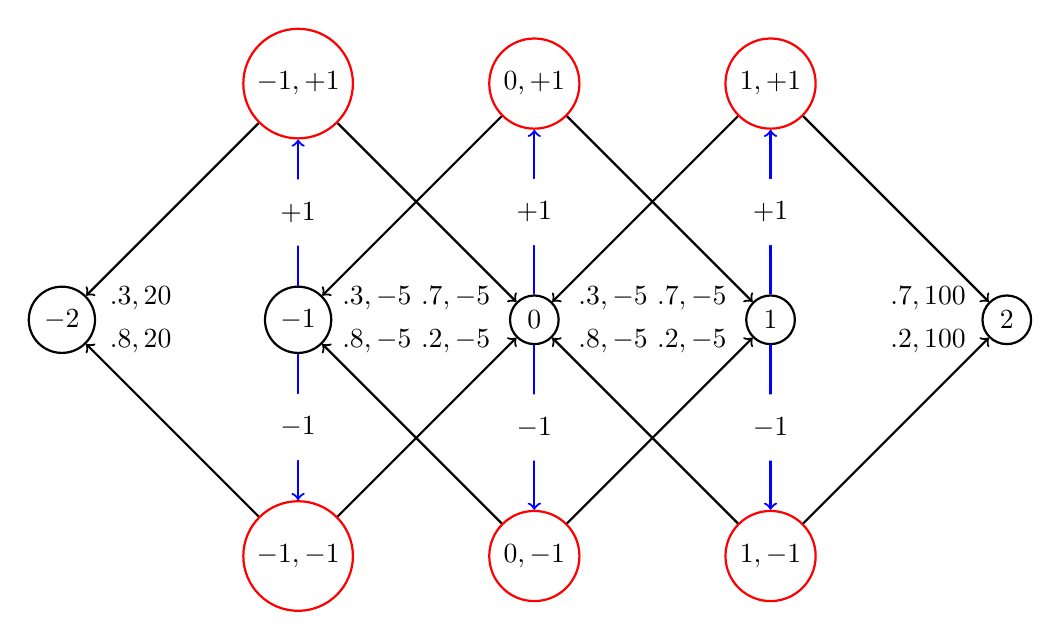
\begin{tikzpicture}
			\begin{scope}[every node/.style={circle,thick,draw}]
	    		\node (-2) at (0,0) {$-2$};
	    		\node (-1) at (3,0) {$-1$};
	    		\node (0) at (6,0) {$0$};
	    		\node (1) at (9,0) {$1$};
	    		\node (2) at (12,0) {$2$};
			\end{scope}
			\begin{scope}[every node/.style={circle,thick,draw=red}]
	    		\node (A) at (3,3) {$-1,+1$};
	    		\node (B) at (6,3) {$0,+1$};
	    		\node (C) at (9,3) {$1,+1$};
	    		\node (D) at (3,-3) {$-1,-1$};
	    		\node (E) at (6,-3) {$0,-1$};
	    		\node (F) at (9,-3) {$1,-1$};
			\end{scope}
	
			\begin{scope}[every node/.style={fill=white,circle},every edge/.style={draw=blue,thick}]
				\path [->] (-1) edge node {$+1$} (A);	    		
	    		\path [->] (0) edge node {$+1$} (B);
	    		\path [->] (1) edge node {$+1$} (C);
	    		\path [->] (-1) edge node {$-1$} (D);	    		
	    		\path [->] (0) edge node {$-1$} (E);
	    		\path [->] (1) edge node {$-1$} (F);
			\end{scope}
			\begin{scope}[every edge/.style={draw=black,thick}]
				\path [->] (A) edge node {} (0);	    		
	    		\path [->] (B) edge node {} (1);
	    		\path [->] (C) edge node {} (2);
	    		\path [->] (A) edge node {} (-2);	    		
	    		\path [->] (B) edge node {} (-1);
	    		\path [->] (C) edge node {} (0);
	    		\path [->] (D) edge node {} (-2);	    		
	    		\path [->] (E) edge node {} (-1);
	    		\path [->] (F) edge node {} (0);
	    		\path [->] (D) edge node {} (0);	    		
	    		\path [->] (E) edge node {} (1);
	    		\path [->] (F) edge node {} (2);
			\end{scope}
			\begin{scope}[]
	    		\node [above] at (1,0) {$.3,20$};
	    		\node [above] at (4,0) {$.3,-5$};
	    		\node [above] at (7,0) {$.3,-5$};
	    		\node [above] at (5,0) {$.7,-5$};
	    		\node [above] at (8,0) {$.7,-5$};
	    		\node [above] at (11,0) {$.7,100$};
	    		\node [below] at (1,0) {$.8,20$};
	    		\node [below] at (4,0) {$.8,-5$};
	    		\node [below] at (7,0) {$.8,-5$};
	    		\node [below] at (5,0) {$.2,-5$};
	    		\node [below] at (8,0) {$.2,-5$};
	    		\node [below] at (11,0) {$.2,100$};
			\end{scope}
		\end{tikzpicture}
	\end{center}
	
	$$V_{opt}^{(t)}(s) = max_{a \in actions(s)} \sum_{s'} T(s,a,s')[reward(s,a,s') + \gamma V_{opt}^{(t-1)}(s')]$$	
	
	Iteration 0:\\
	\begin{tabular}{c | c c c c c}
		$s$ & $-2$ & $-1$ & $0$ & $1$ & $2$ \\
  		$V_{opt}$ & $0$ & $0$ & $0$ & $0$ & $0$ \\
  		$\pi_{opt}$ & $none$ & $none$ & $none$ & $none$ & $none$ \\
	\end{tabular}
  
  \begin{align*}
  		V_{opt}^{(1)}(-1) &= max(.7(-5 + 1(0)) + .3(20 + 1(0)), .8(20 + 1(0)) + .2(-5 + 1(0))) = 15\\
  		V_{opt}^{(1)}(0) &= max(.7(-5 + 1(0)) + .3(-5 + 1(0)), .8(-5 + 1(0)) + .2(-5 + 1(0))) = -5\\
  		V_{opt}^{(1)}(1) &= max(.7(100 + 1(0)) + .3(-5 + 1(0)), .8(-5 + 1(0)) + .2(100 + 1(0))) = 68.5
	\end{align*}
	
	Iteration 1:\\
	\begin{tabular}{c | c c c c c}
		$s$ & $-2$ & $-1$ & $0$ & $1$ & $2$ \\
  		$V_{opt}$ & $0$ & $15.0$ & $-5.0$ & $68.5$ & $0$ \\
  		$\pi_{opt}$ & $none$ & $-1$ & $either$ & $+1$ & $none$ \\
	\end{tabular}
	
	\begin{align*}
  		V_{opt}^{(2)}(-1) &= max(.7(-5 + 1(-5)) + .3(20 + 1(0)), .8(20 + 1(0)) + .2(-5 + 1(-5))) = 14\\
  		V_{opt}^{(2)}(0) &= max(.7(-5 + 1(68.5)) + .3(-5 + 1(15)), .8(-5 + 1(15)) + .2(-5 + 1(68.5))) = 47.45\\
  		V_{opt}^{(2)}(1) &= max(.7(100 + 1(0)) + .3(-5 + 1(-5)), .8(-5 + 1(-5)) + .2(100 + 1(0))) = 67
	\end{align*}
	
	Iteration 2:\\
	\begin{tabular}{c | c c c c c}
		$s$ & $-2$ & $-1$ & $0$ & $1$ & $2$ \\
  		$V_{opt}$ & $0$ & $14.0$ & $47.45$ & $67.0$ & $0$ \\
  		$\pi_{opt}$ & $none$ & $+1$ & $+1$ & $+1$ & $none$ \\
  	\end{tabular}

\end{enumerate}

\section*{\normalsize Problem 2: Transforming MDPs}

Let's implement value iteration to compute the optimal policy on an arbitrary MDP. Later, we'll create the specific MDP for Blackjack. 
\smallskip

\begin{enumerate}[label=(\alph*)]

  \item If we add noise to the transitions of an MDP, does the optimal value always get worse? Specifically, consider an MDP with reward function $Reward(s,a,s')$, states $States$, and transition function $T(s,a,s′)$. Let's define a new MDP which is identical to the original, except that on each action, with probability $\frac{1}{2}$, we randomly jump to one of the states that we could have reached before with positive probability. Formally, this modified transition function is:
  
  $$T'(s,a,s') = \frac{1}{2} T(s,a,s') + \frac{1}{2} \frac{1}{| \{ s'':T(s,a,s'')>0 \} |}$$
  
  Let $V_1$ be the optimal value function for the original MDP, and $V_2$ the optimal value function for the modified MDP. Is it always the case that $V_1(s_{start}) \geq V_2(s_{start})$? If so, prove it on the written portion and put return None for each of the code blocks. Otherwise, construct a counter example by filling out \texttt{CounterexampleMDP} in \texttt{submission.py}.
  
  This is not always the case. Here is a counterexample.
  
  \begin{center}
	  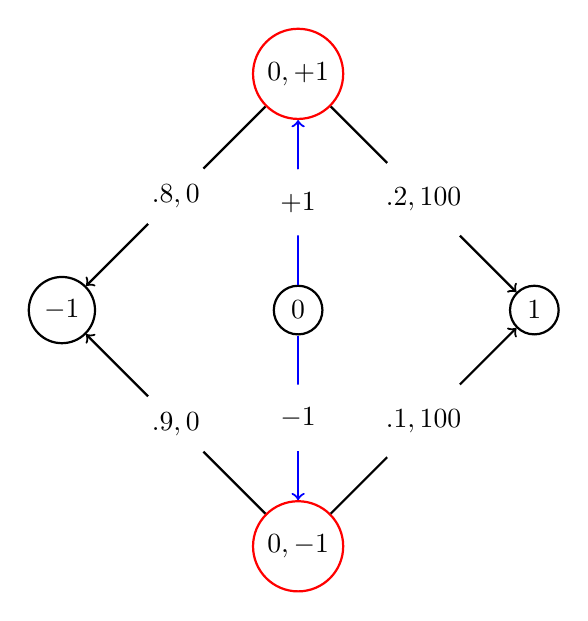
\begin{tikzpicture}
			\begin{scope}[every node/.style={circle,thick,draw}]
	    		\node (-1) at (3,0) {$-1$};
	    		\node (0) at (6,0) {$0$};
	    		\node (1) at (9,0) {$1$};
			\end{scope}
			\begin{scope}[every node/.style={circle,thick,draw=red}]
	    		\node (A) at (6,3) {$0,+1$};
	    		\node (B) at (6,-3) {$0,-1$};
			\end{scope}
	
			\begin{scope}[every node/.style={fill=white,circle},every edge/.style={draw=blue,thick}]
				\path [->] (0) edge node {$+1$} (A);	    		
	    		\path [->] (0) edge node {$-1$} (B);
			\end{scope}
			\begin{scope}[every node/.style={fill=white,circle},every edge/.style={draw=black,thick}]
				\path [->] (A) edge node {$.2,100$} (1);	    		
	    		\path [->] (A) edge node {$.8,0$} (-1);
	    		\path [->] (B) edge node {$.1,100$} (1);
	    		\path [->] (B) edge node {$.9,0$} (-1);
			\end{scope}
		\end{tikzpicture}
	\end{center}
	
	\begin{tabular}{c | c c c}
		$s$ & $-1$ & $0$ & $1$\\
  		$V_1$ & $0$ & $20$ & $0$\\
  		$V_2$ & $0$ & $35$ & $0$\\
  	\end{tabular}
  
  \item Suppose we have an acyclic MDP for which we want to find the optimal value at each node. We could run value iteration, which would require multiple iterations -- but it would be nice to be more efficient for MDPs with this acyclic property. Briefly explain an algorithm that will allow us to compute $V_{opt}$ for each node with only a single pass over all the $(s,a,s')$ triples.
  
  The alogrithm would involve calculating $V_{opt}$ for the end states and working backwards to the start state.
  
  \item Suppose we have an MDP with states $States$ and a discount factor $\gamma < 1$, but we have an MDP solver that can only solve MDPs with discount factor of 1. How can we leverage the MDP solver to solve the original MDP?
  
  Let us define a new MDP with states $States'= States \cup \{o\}$, where $o$ is a new state. Let's use the same actions $Actions'(s) = Actions(s)$, but we need to keep the discount $\gamma' = 1$. Your job is to define new transition probabilities $T'(s,a,s')$ and rewards $Reward'(s,a,s')$ in terms of the old MDP such that the optimal values $V_{opt}(s)$ for all $s \in States$ are equal under the original MDP and the new MDP.
  
  Hint: If you're not sure how to approach this problem, go back to the notes from the first MDP lecture and read closely the slides on convergence, toward the end of the deck.
  
  From the notes: ``We can reinterpret the discount $\gamma < 1$ condition as introducing a new transition from each state to a special end state with probability $(1 - \gamma)$, multiplying all the other transition probabilities by $\gamma$, and setting the discount to 1. The interpretation is that with probability $1 - \gamma$, the MDP terminates at any state."
  
  \begin{align*}
  		T'(s,a,s') &= \gamma T(s,a,s')\\
  		Rewards'(s,a,s') &= Rewards(s,a,s')
  \end{align*}

\end{enumerate}

\section*{\normalsize Problem 3: Peeking Blackjack}

\begin{enumerate}[label=(\alph*)]

  \item coding
  
  \item coding
		
\end{enumerate}

\section*{\normalsize Problem 4: Learning to Play Blackjack}

So far, we've seen how MDP algorithms can take an MDP which describes the full dynamics of the game and return an optimal policy. But suppose you go into a casino, and no one tells you the rewards nor the transitions. We will see how reinforcement learning can allow you to play the game and learn its rules and strategy at the same time!

\begin{enumerate}[label=(\alph*)]

  \item coding
  
  \item Now let's apply Q-learning to an MDP and see how well it performs in comparison with value iteration. First, call \texttt{simulate} using your Q-learning code and the \texttt{identityFeatureExtractor()} on the MDP \texttt{smallMDP} (defined for you in \texttt{submission.py}), with 30000 trials and default \texttt{explorationProb}.
  
  How does the Q-learning policy compare with a policy learned by value iteration (i.e., for how many states do they produce a different action)? (Don't forget to set the \texttt{explorationProb} of your Q-learning algorithm to 0 after learning the policy.) Now run \texttt{simulate()} on \texttt{largeMDP}, again with 30,000 trials. How does the policy learned in this case compare to the policy learned by value iteration? What went wrong?
  
  Q-learning and value iteration performed similarly on \texttt{smallMDP}. Approximately 3\% of the states were assigned differing actions. Q-learning did not perform as well on \texttt{largeMDP}. About 30\% of the states were assigned differing actions. There were many more states in \texttt{largeMDP}, and the feature extractor \texttt{identityFeatureExtractor} is not good at generalizing.
  
  \item coding
  
  \item Sometimes, we might reasonably wonder how an optimal policy learned for one MDP might perform if applied to another MDP with similar structure but slightly different characteristics. For example, imagine that you created an MDP to choose an optimal strategy for playing "traditional" blackjack, with a standard card deck and a threshold of 21. You're living it up in Vegas every weekend, but the casinos get wise to your approach and decide to make a change to the game to disrupt your strategy: going forward, the threshold for the blackjack tables is 17 instead of 21. If you continued playing the modified game with your original policy, how well would you do? (This is just a hypothetical example; we won't look specifically at the blackjack game in this problem.)

	To explore this scenario, let's take a brief look at how a policy learned using value iteration responds to a change in the rules of the MDP.

	\begin{itemize}
		\item First, run value iteration on the \texttt{originalMDP} (defined for you in \texttt{submission.py}) to compute an optimal policy for that MDP.
		\item Next, simulate your policy on \texttt{newThresholdMDP} (also defined for you in \texttt{submission.py}) by calling simulate with an instance of \texttt{FixedRLAlgorithm} that has been instantiated using the policy you computed with value iteration. What is the expected reward from this simulation? Hint: read the documentation (comments) for the \texttt{simulate} function in util.py, and look specifically at the format of the function's return value.
		\item Now try simulating Q-learning on \texttt{originalMDP} (30,000 trials). Then, using the learned parameters, run Q-learning again on \texttt{newThresholdMDP} (again, 30000 trials). What is your expected reward under the new Q-learning policy? Provide some explanation for how the rewards compare with when \texttt{FixedRLAlgorithm} is used. Why they are different?
		
		(Below is the previous version of this problem. If you have followed this one, it is okay. You don't have to change your solution. But the correct way to observe the difference is following the above procedure;

		Now try simulating Q-learning directly on \texttt{newThresholdMDP} instead. What is your expected reward under the new Q-learning policy? Provide some explanation for how the rewards compare, and why they are different.) 
	\end{itemize}
	
	See code. Following the original value iteration optimum policy, the expected reward is low when the MDP is altered. A similar result is seen with Q-learning if no exploration is allowed when run on the new MDP. If exploration is allowed, Q-learning performs superiorly and returns an expected reward that is close to that when following the optimum policy of the new MDP.
		
\end{enumerate}

\end{document}
